
	\documentclass{article}
	\usepackage{amsmath,amssymb}
	\usepackage[inline]{enumitem}
	\usepackage{blindtext}
	\usepackage{booktabs}
	\usepackage{graphicx}
	\usepackage{xcolor}
	\usepackage[vmargin = 1.5in, top = 1in, bottom = 1.2in, letterpaper]{geometry}
	\usepackage{listings}
	\usepackage{courier}
	\usepackage{multicol}
	\usepackage{multirow}
	\usepackage{bm}
	\usepackage{algorithm}
	\usepackage{algpseudocode}
	\usepackage{subfigure}
	\lstset{
	basicstyle = \small\tt,
	keywordstyle = \ttfamily\bfseries\color{blue},
	commentstyle = \it\color[cmyk]{1,0,1,0},
	stringstyle = \tt\color[RGB]{128,0,0},
	%frame = single,
	backgroundcolor = \color[RGB]{245,245,244},
	breaklines,
	extendedchars = false,
	xleftmargin = 2em,
	xrightmargin = 2em,
	aboveskip = 1em,
	tabsize = 4,
	showspaces = false
	showstringspaces = false
	}

	\setlength{\parindent}{0em}
	\setlength{\parskip}{1em}
	\begin{document}
	
	% \newfontfamily\courier{Courier New}

	
	\title{\bf STAT 580 Final Report}
	\author{Yifan Zhu, Gang Han, Lijin Zhang, Lingnan Yuan\\ \  \\ \textit{Department of Statistics, Iowa State University}}
	\date{}
	\maketitle
	
	\section{Summary of Soft-Impute}

	\cite{hastie2015statistical, mazumder2010spectral}
	\section{Comparison of SVD implementations}
	\section{Application}
	\subsection{Lena}
	Based the comparison between these 4 implementations, we choose the \verb|original svd| in R to do the image imputing. The reason is that from {\color{red}Figure} we can see the \verb|original svd| and \verb|rcpparmadillo| seems to be more steady than \verb|irlba| (the gray region that represents confidence interval is smaller). Also these two methods seems to have smaller test error around the true matrix rank. Because the data for lena is not large, thus we do not care about the speed of implementations. And we can expect \verb|original svd| and \verb|rcpparmadillo| would give almost the same results from the comparison part, hence we choose to use \verb|orginal svd|. 

	First we randomly removed the 40\% of the lena and got an image with only 60\% being observed. Now we use the 60\% as our data to restore the image with soft-impute. In order to obtain an optimal restoration, we need to tune the parameter $\lambda$ in the soft-impute algorithm. The strategy we took is to further divide the data into two parts: 70\% as training data and 30\% as validation data. We did the imputation with a series of $\lambda$'s (we used $\lambda = 500, 490, \ldots, 10$). Then we compared the corresponding validation part of these imputed matrix with the true validation set. The error term we used is
	\begin{equation}\label{valid_error}
	\frac{\|P_{\Omega_{\rm validation}}(Z_{\rm true} - \hat{Z}_{\lambda})\|^2_{F}}{\|P_{\Omega_{\rm validation}} Z_{\rm true}\|_{F}^2}
	\end{equation}
	where $\Omega_{\rm validation}$ is the set of matrix entries that validation set has.

	We chose the $\lambda$ that gave us the smallest test error and applied soft-impute again on the whole data set with the optimal $\lambda$ we got. In this case, with the test error we defined, the optimal $\lambda$ we chose is $\lambda = 190$. 

	After we imputed the matrix, we wanted to see how close it is to the true one. We looked at the rank of recovered matrix and the true matrix, and also the error of the imputed one compared with the true one. The error we used is 
	\begin{equation} \label{test_error}
	\frac{\|P_{\Omega_{\rm test}}(Z_{\rm true} - \hat{Z}_{\lambda})\|_{F}^2}{\|P_{\Omega_{\rm test}}(Z_{\rm true})\|_F^2} 
	\end{equation}
	where $\Omega_{\rm test}$ is the set of matrix entries that test set has, which is the rest 40\% of the true lena image that is not taken as data.

	With the optimal $\lambda$, the rank of recovered matrix is
	\[\textrm{rank} (\hat{Z}_{\lambda_{\rm opt}}) = 77\]
	While the true rank is
	\[\textrm{rank}(Z_{\rm true}) = 254\]

	The test error of the imputed matrix when compared with the true matrix in the rest 40\% of the image is  
	\[\textrm{test error} = 0.031\]

	Finally, we compare the true image, incomplete image and the restored image visually, which is shown in Figure \ref{lena}.
	\begin{figure}[!htb]
    \centering
    \subfigure[true image]{
            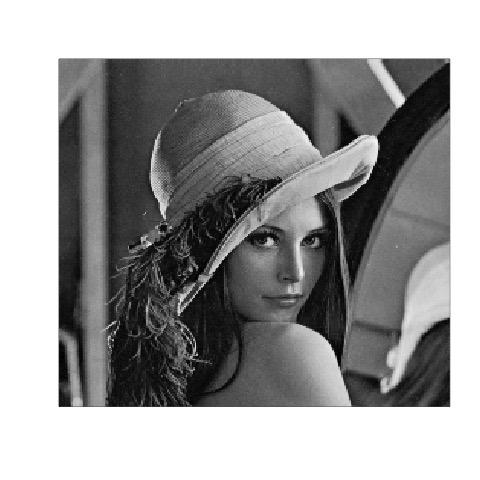
\includegraphics[width=1.8in]{lena_true.jpg}

    }
    ~ 
    \subfigure[incomplete image]{
        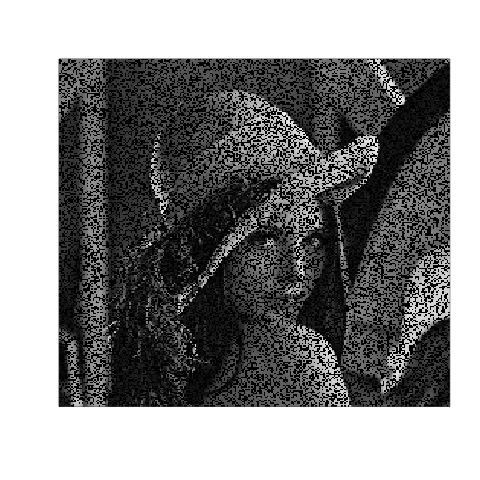
\includegraphics[width=1.8in]{lena_data.jpg}
}
     ~ 
    \subfigure[restored image]{
        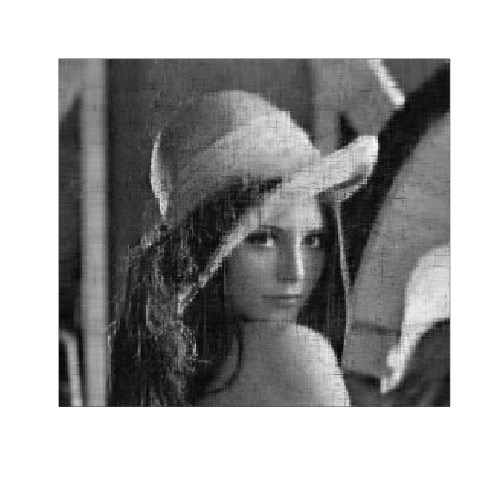
\includegraphics[width=1.8in]{lena_restored}
    }
    \caption{Visually comparing the imputed image with the true one}
    \label{lena}
\end{figure}
	
	We can see that the restored image is not so good. It is not like a natural image with good smoothness. Also the restored image has a much smaller rank than the true one. However, soft-impute is intended to impute low-rank matrix, and true image actually has a quite big rank. That might also be a reason why the final result is not good.

	\subsection{MovieLens}

	In this section, we use MovieLen 100K Dataset to apply our soft-impute algorithm. As the data set is not complete when we convert the original data into a matrix form, we need to divide it into three parts: 70\% as training set, 15\% as validation set and 15\% as test set. What we did is similar as we did in lena part. We first use the training set as observed entries to impute the matrix, then we compare the validation set with the corresponding entries of the imputed matrix. Again we use (\ref{valid_error}) as the error term and we pick the $\lambda$ with the smallest validation error. After we obtained the optimal $\lambda$, we use the 70\% training set and 15\% validation set combined as our data, or observed entries to impute the matrix. Then we compare the test set with the corresponding entries of the imputed matrix and calculate the test error using (\ref{test_error}). Besides, we calculated the RMSE of the imputed matrix with respect to the test set in corresponding parts. The RMSE formula is
	\begin{equation}
	\textrm{RMSE} = \sqrt{\frac{\|P_{\Omega_{\rm test}}(Z_{\rm true} - \hat{Z}_{\lambda_{\rm opt}})\|_{F}^2}{|\Omega_{\rm test}|}}
	\end{equation}

	As the dataset is pretty big, we chose \verb|irlba| and \verb|rcpparmadillo| as two implementations to be applied to this dataset. There two implementations are relatively faster than others ,thus with the big dataset we could save a lot of time. 

	In choosing the optimal $\lambda$, as the big matrix takes time to impute, we used a strategy to find the optimal one using 3 grids of $\lambda$'s by assuming the test error as a function of $\lambda$ is unimodal. The first grid is $\lambda = 100, 90, \ldots, 10$ with step size 10. From this grid we can find the interval where the optimal $\lambda$ located. We found $\lambda  = 10$ was the smallest in this grid. Then we knew the optimal $\lambda$ is between $20$ and $0$. Then we used the second grid $\lambda = 19, 16, \ldots, 4, 1$ with step size 3. We found $\lambda = 13$ is the smallest in this grid. Then we tried the third grid $\lambda = 15, 14, 12, 11$. In this grid, $\lambda = 12$ gave us the smallest test error. But comparing it with the test error when $\lambda = 13$, we found the test error for $\lambda =13$ was smaller. Hence, the optimal $\lambda$ we chose is $\lambda = 13$. 





	

	\newpage

	\bibliographystyle{unsrt}
	\bibliography{reference}

	
	\end{document}